\documentclass{l4proj}

%
%  Macro files
%  Originally from Frisch, Castagna, Benzaken
%  
%

%% Ornela
\newcommand{\abstr}[4]{\lambda_{({#1} , {#2})} {#3}.{#4}}
\newcommand{\semval}[2]{\sem{#1}_{\mathcal #2}}



\newif{\ifSHORT}
\newif{\ifLongVersion}
\newif{\ifWithRecords}
\newif{\ifWiths}

\newcommand{\possiblecut}[1]{{\color{black}#1}}   

\newcommand{\maincomment}[1]{%
  \ifMarginalComments{\mbox{}\\[1mm]$\Longrightarrow$\textsf{#1}\mbox{}\\[1mm]} \else {} \fi}

\newenvironment{mylist}{%
\begin{list}{$\bullet$}{\topsep2pt\parskip0pt\partopsep0pt\itemsep3pt\labelwidth10.5mm\labelsep3pt\leftmargin11mm}}%
{\end{list}}

%
%  unsemplice comando che mi dice la versione
%
\usepackage{calc}\newcounter{tempo}\setcounter{tempo}{\time}
\newcommand{\version}[1]{\mbox{}\\[-\baselineskip]%
   \raisebox{#1in}[0in][0in]{\makebox[\textwidth][c]{\rm\small \today:v.\thetempo}}}
\newcommand{\titlepageheader}[1]{\mbox{}\\[-\baselineskip]%
\raisebox{5.3in}[0in][0in]{\makebox[\textwidth][c]{\rm\small #1}}}
\newcommand{\duce}{$\mathbb{C}$Duce }
\newcommand{\cduce}{$\mathbb{C}$Duce }
\newcommand{\cdoge}{$\mathbb{C}$Doge }
\newcommand{\cpi}{$\mathbb{C}\pi$ }
\newcommand{\cobj}{$\mathbb{C}$Obj }
\newcommand{\sempi}{$\pi_\leq$}   % was semantic-$\pi${}}
\newcommand{\emptyl}{\mathsf{empty}}
%
% Daniele
%
% altri commandi
\newcommand{\wt}[1]{\widetilde{#1}}

\newcommand{\synrnd}{\mathbf{rnd}}
\newcommand{\synclass}{\mathbf{class} \ }
\newcommand{\syninterface}{\mathbf{interface} \ }
\newcommand{\synext}{\ \mathbf{extends }\ }
\newcommand{\synimpl}{\ \mathbf{implements}\ }
\newcommand{\synret}{\mathbf{return}\ }
\newcommand{\synthis}{\mathbf{this}}
\newcommand{\synsuper}{\mathbf{super}}
\newcommand{\synfinal}{\mathbf{final}}
\newcommand{\synnew}{\mathbf{new}\ }
\newcommand{\syndecl}[3]{\synclass #1 \synext #2\ \{#3\}}
\newcommand{\synidecl}[2]{\synclass #1 \synext #2\ }

\newcommand{\mmif}{\mathbf{if}}
\newcommand{\mmthen}{\mathbf{then}}
\newcommand{\mmelse}{\mathbf{else}}
\newcommand{\mmclass}{\mathbf{class}}
\newcommand{\mmnew}{\mathbf{new}}
\newcommand{\mmnull}{\mathbf{null}}
\newcommand{\mmextends}{\mathbf{extends}}
\newcommand{\mmint}{\mathbf{int}}
\newcommand{\mmreal}{\mathbf{real}}
\newcommand{\mmbool}{\mathbf{bool}}
\newcommand{\mmtrue}{\mathbf{true}}
\newcommand{\mmfalse}{\mathbf{false}}
\newcommand{\nname}{\mathbf{name}}
\newcommand{\mmreturn}{\mathbf{return}}
\newcommand{\mminstof}{\mathbf{instanceof}}
\newcommand{\mmtry}{\mathbf{try}}
\newcommand{\mmcatch}{\mathbf{catch}}
\newcommand{\mmthrow}{\mathbf{throw}}
\newcommand{\mmlet}{\mathbf{let}}
\newcommand{\mmin}{\mathbf{in}}
\newcommand{\nominal}{\mathbf{nominal}}

\newcommand{\naming}[1]{(#1)^\nname}
\newcommand{\type}{\mathit{type}}
\newcommand{\mbody}{\mathit{body}}
\newcommand{\judge}[2]{#1 \vdash #2}
\newif\ifmai\maifalse


\newcommand{\height}[1]{\hslash(#1)}%{\textit{height}(#1)}
%\DeclareMathOperator{\uparrowop}{\uparrow}
%\DeclareMathOperator{\downarrowop}{\downarrow}
%
% definition enum environment
%
\newenvironment{enum}{\begin{enumerate}\vspace{-5pt}\topsep0pt\parskip0pt\partopsep0pt\itemsep1pt}{\end{enumerate}\vspace{-5pt}}


%
%
\newcommand{\A}{{\cal A}}
\newcommand{\Norm}{{\cal N}}
\newcommand{\exten}{\mathbb E}
\newcommand{\extenf}{\mathbb{E}_f}
\newcommand{\atoms}{{\mathbb T}}
\newcommand{\myitem}{\mbox{}\\[.5mm]\hspace*{3.5mm}--~~}

\newcommand{\dead}{\textsf{0}}
%\newcommand{\mathbb}[1]{\Bbb{#1}}
%\newcommand{\llbracket}{[\![}
%\newcommand{\rrbracket}{]\!]}

\newcommand{\VAR}{\textit{Var}}
\newcommand{\zero}{\mathbf{0}}
\newcommand{\one}{\mathbf{1}}
%\newcommand{\qed}{\mbox{}\hfill\mbox{$\Box$}}
\newcommand{\bij}{\partial}
\newcommand{\para}{~~|~~}
\newcommand{\hasse}[1]{\xymatrix@R-1em@C-2em{#1}}

\newcommand{\todo}[1]{{\bf \underline{TODO:} #1}}
\newcommand{\ignore}[1]{}
\newcommand{\Is}{\colon\!\!\colon \!\!\!\!= }

\newcommand{\txtvee}{\text{\rm ~or~}}
\newcommand{\txtwedge}{\text{\rm ~and~}}

\newcommand{\dom}{\textit{dom}}

%\newcommand{\naturals}{\mathbb{N}}

% Op�rateurs math�matiques
\renewcommand{\P}{{\cal P}}
\newcommand{\Pf}{{\P_f}}
\newcommand{\compl}[2]{{\complement_{#2}} {#1}}
\newcommand{\egdef}{\stackrel{\textrm{\tiny def}}{=}}
\newcommand{\segdef}{\!\!\!\stackrel{\textrm{\tiny def}}{=}\!\!\!}
\renewcommand{\subset}{\subseteq}
\renewcommand{\emptyset}{\varnothing}

\newcommand{\cX}{{\cal X}}

% Les univers
\newcommand{\ubasic}{{\text{\bf basic}}}
\newcommand{\urec}{{\text{\bf rec}}}
\newcommand{\ufun}{{\text{\bf fun}}}

% Basic types
\newcommand{\btypes}{{\mathbb B}}
\newcommand{\semb}[1]{{\cal B} {\llbracket #1 \rrbracket}}
\newcommand{\Types}{\textbf{Types}}
% Les mod�les
\newcommand{\domaine}{{\cal D}}
%\newcommand{\univ}{{\cal U}}
\newcommand{\domwr}{\domaine_\Omega}
\newcommand{\stdmod}{{\cal U}}
\newcommand{\stdmodwr}{{\cal U}_\Omega}
\newcommand{\sem}[1]{{\llbracket #1 \rrbracket}}
\newcommand{\esem}[1]{{\mathbb E}\left( #1 \right)}
\newcommand{\esemd}[1]{{\mathbb E}$D$}
\newcommand{\esemp}[1]{{\cal E}\llparenthesis #1 \rrparenthesis}
\newcommand{\tsem}[1]{\llparenthesis #1 \rrparenthesis}
%\newcommand{\semv}[1]{{\mathbb V}{\llbracket #1 \rrbracket}}


% Les types
\newcommand{\functor}{{\mathbb T}}
\newcommand{\syntypes}{{\mathcal{T}}}
\newcommand{\atomtypes}{\textit{A\/}}%{\syntypes^\circ}
\newcommand{\synatoms}{{\mathcal A}}
\newcommand{\synprod}{\pmb{\times}}
\newcommand{\synarrow}{\pmb{\rightarrow}}
\newcommand{\synneg}{\pmb{\neg}}
\newcommand{\synvee}{\pmb{\vee}}
\newcommand{\synwedge}{\pmb{\wedge}}
\newcommand{\syndiff}{\pmb{\backslash}}
\newcommand{\syncap}{\operatornamewithlimits{\pmb{\bigwedge}}}
\newcommand{\syncup}{\operatornamewithlimits{\pmb{\bigvee}}}
\newcommand{\socle}[1]{\beth(#1)}
\newcommand{\appl}{\bullet}
\newcommand{\synch}[2]{\textit{ch}^{#1}\!(#2)}
\newcommand{\synchan}[1]{\textit{ch}(#1)}
\newcommand{\synchanK}{\textit{ch}}
\newcommand{\synchanout}[1]{\textit{ch}^{\!\textbf{--}\!\!}(#1)}
\newcommand{\synchanin}[1]{\textit{ch}^+(#1)}

%blackboardbold types
\def\bbbone{{\mathchoice {\rm 1\mskip-4mu l} {\rm 1\mskip-4.5mu l}
          {\rm 1\mskip-4.5mu l} {\rm 1\mskip-5mu l}}}
\newcommand{\synnatone}{\bbbone}
\newcommand{\synnatk}{\Bbbk}
\newcommand{\synnat}[1]{\mathbb{#1}}

% Les motifs
\newcommand{\pator}[2]{#1 \pmb{|} #2}
\newcommand{\patand}[2]{#1 \pmb{\wedge} #2}
%\newcommand{\patleft}[1]{\pmb{(}#1\pmb{,\_)}}
%\newcommand{\patright}[1]{\pmb{(\_,}#1\pmb{)}}
\newcommand{\patcst}[2]{\pmb{(}#1\pmb{:=}#2\pmb{)}}
\newcommand{\patpair}[2]{\pmb{(}#1\pmb{,}#2\pmb{)}}

% Filtrage
\newcommand{\erreur}{\Omega}
\newcommand{\accept}[1]{\pmb{\lbag} #1 \pmb{\rbag}}
\newcommand{\acceptd}[1]{\pmb{\lfloor} #1 \pmb{\rfloor}}
\newcommand{\semaccept}[1]{\Lbag #1 \Rbag}
\newcommand{\filter}[2]{({#1}/{#2})}%{ ({#1} \Downarrow {#2}) }
\newcommand{\semfilter}[2]{ ({#1} \downarrow {#2}) }


% Symboles du langage
%\newcommand{\myarrow}{\Pisymbol{cmt}{61}\Pisymbol{pcr}{62}}%
\newcommand{\myarrow}{\!\!\boldsymbol{\Rightarrow}\!\!} %\texttt{\char61\char62\relax}}
\newcommand{\mybar}{\texttt{|}}%
\newcommand{\motifs}{\mathbb{P}}
\newcommand{\vars}{\mathbb{V}}
\newcommand{\consts}{\mathbb{C}}
\newcommand{\exprs}{{\mathbb E}}
\newcommand{\expr}{{e}}
\newcommand{\pat}{{\tt p}}
\newcommand{\const}{{n}}
\newcommand{\op}{{o}}
\newcommand{\ops}{{\mathbb O}}
\newcommand{\valeurs}{{\cal V}}
\newcommand{\values}{\valeurs}
\newcommand{\blpar}{\boldsymbol{(}}
\newcommand{\brpar}{\boldsymbol{)}}
\newcommand{\match}[5]{\mathtt{match~} #1 \mathtt{~with~} #2 \myarrow #3 \mybar
  #4 \myarrow #5}
\newcommand{\typecase}[5]{\mathtt{typecase~} #1 \mathtt{~with~} (#2 :
  #3) \myarrow #4 \mybar (#2 : \synneg #3) \myarrow #5}
\newcommand{\typec}[5]{\texttt{(} #3=#1\pmb{\in}#2\texttt{)}\pmb{?}#4\texttt{{:}}#5}
\newcommand{\genabstraction}[3]{\abstr{f}{#1}{#2}{#3}}
%\newcommand{\abstr}[4]{\boldsymbol{\mu} #1^{\blpar #2 \brpar}\blpar #3 \brpar \boldsymbol{.}#4}
\newcommand{\stdmatch}{\match{\expr}{p_1}{\expr_1}{p_2}{\expr_2}}
\newcommand{\exprpair}[2]{\blpar #1 \boldsymbol{,} #2 \brpar}
\newcommand{\exprop}[2]{#1 \blpar #2 \brpar}

% S�mantique op�rationnelle
%\newcommand{\wrong}{\mbox{\bf wrong}}
\newcommand{\wrong}{\Omega}
%\newcommand{\reject}{\mbox{\bf reject}}
%\newcommand{\apply}{{\tt apply}}


% Enregistrements
\newcommand{\domdef}[1]{\text{Def}(#1)}
\newcommand{\labels}{{\cal L}}
\newcommand{\urecord}{{\text{\bf record}}}
\newcommand{\trec}[2]{\pmb{[} #1 : #2 \pmb{]}}
\newcommand{\tsupp}[1]{\text{\bf S}(#1)}
%\newcommand{\supp}[1]{\text{Supp}(#1)}
\newcommand{\patrec}[2]{\{ #1 : #2\}}
\newcommand{\Iff}{\Longleftrightarrow}
\newcommand{\reff}{\mathtt{ref}\,}
\newcommand{\lazy}{\mathtt{lazy}\,}


% Th�or�mes ...
%\newtheorem{theorem}{Theorem}[section]
%\newtheorem{lemma}[theorem]{Lemma}
%\newtheorem{proposition}[theorem]{Proposition}
%\newtheorem{corollary}[theorem]{Corollary}
%\newtheorem{definition}[theorem]{Definition}
%\newtheorem{condition}{Condition}
%\newenvironment{definition}{\begin{defn}}{\qed\end{defn}}
%\newtheorem{definition}[theorem]{Definition}
%\newtheorem{property}[theorem]{Property}
%\newtheorem{convention}[theorem]{Convention}
%\newtheorem{remark}[theorem]{Remark}
%\renewenvironment{proof}{{\sl Proof}:}{\qed}

\usepackage{amsmath, amssymb}
\usepackage{float}
\usepackage{changepage}

\SetKwRepeat{Do}{do}{while}
\SetKwProg{Fn}{Function}{:}{end}


\begin{document}

%===================================================================================================

\title{SFJ - Boolean types and semantic subtyping for Featherweight Java}
\author{Artem Usov}
\date{April 6, 2020}

\maketitle

%===================================================================================================

\begin{abstract}
    The type system of a programming language often dictates its safety and expressivity.
    There are two distinct approaches to defining a type system: the \emph{syntactic} and \emph{semantic}.
    In the semantic approach, one defines a model of the language and an interpretation of types as subsets of this model.
    Subtyping is defined as inclusion of subsets denoting types.
    \vskip 0.5em
    In this paper we present SFJ---Semantic Featherweight Java, an extension of Featherweight Java, which implements such a semantic type system defined by \cite{Dardha2013, Dardha2017}.
    We further exploit it to integrate boolean types as well as nominal and structural subtyping.
    This paper illustrates the benefits of such language constructs by allowing us to write programs that have higher guarantees of correctness by increasing the static type-checking power of the language whilst being more intuitive at the same time.
\end{abstract}

%===================================================================================================

\renewcommand{\abstractname}{Acknowledgements}

\begin{abstract}
    I would like to thank my supervisor Dr Ornela Dardha for her support and guidance throughout the year as well as her enthusiasm for lecturing which is made interested in programming languages and type systems.
    \vskip 0.5em
    I would also like to thank my parents who have always supported and believed in me.
\end{abstract}

%===================================================================================================

\def\consentname {Artem Usov}
\def\consentdate {6 April 2020}
\educationalconsent

%===================================================================================================

\tableofcontents

%===================================================================================================

\chapter{Introduction}

\pagenumbering{arabic}

\section{End Goal of Programming}

The end goal in all programming projects is to create a solution to the task at hand that exactly solves the initially defined problem and performs exactly as expected by the programmer.
However, this rarely actually happens.

On the one hand, this is often because the original problem is not statically defined.
If, for example, it is a solution for an external client, then their requirements and needs will change over time.
This means the project needs to be adapted over time.
On the other hand, and almost always much less evident, is that programs do not work exactly as the programmer imagines them to work.

In general these are called \emph{bugs} in a program, and have become more and more common as projects and the underlying hardware they run on have become more complex.
Therefore in both academia and industry there have been great efforts over the years to create tools that allow us to decrease the amount of bugs in our programs and increase our productivity.

\subsection{Static Code Analysis}

One area of great effort has been in the development of static code analysis tools.
Some of these exist integrated into the language itself such as with Spark \citep{Carre1990}.
Spark is a formally defined language based on the Ada \citep{Ada1979} language intended for the development of high integrity software such as flight control systems.
Others exist as separate, well-known tools that exist alongside the language such as the Clang analysis tools for C and C++ \footnote{https://clang.llvm.org/docs/ClangTools.html}.

Whilst they are not necessary to write correct programs, these tools have quickly become industry standards for maintaining a level of correctness within codebases and avoiding typical programming errors.

\subsection{How Static Analysis Works}

Underlying how all of the previously mentioned static code analysis tools work, is their use of the \emph{type system} of the language.
Type systems at their most basic work by assigning types to various constructs of a program so that incompatible types cannot be used.

For example, one common area of error in C code that the Clang tools warn about is implicit conversions, where the value of an expression is a different type from the one expected, such as the use of a floating point number where an integer is expected.
The C language will implicitly convert the value to an integer, however this happens unbeknownst to the programmer, which can cause unexpected behaviour later on in the program.
The tools, using their knowledge of the type system that you can only use an integer where an integer is expected, can therefore flag this as being a potential bug.

\section{Varying Type Systems}

The effectiveness of static analysis tools and more generally the \emph{safety} and \emph{expressivity} of a programming language therefore depends on the type system that is uses.
Type systems have evolved from the relatively simple systems in languages like C to more complex ones such as in Java which have class types and subtyping relations where types can be substituted for one another.

More modern advances in type systems include the use of linear types in the Cyclone \citep{grossman2002} language which allows us to more naturally and logically define finite state machines.
There also exist other new developments in type systems such as boolean types which are explored in this paper.

\section{Goals of this Project}

In this section, the issues and aims of this paper are presented.

\subsection{Problem Statement}

The typical hierarchical subtyping definitions in Java quite often restrict and complicate the logic that the programmer wants to implement.
These problems come up particularly often when working with legacy code which has incorrectly defined abstractions in its classes.
This therefore leads to less understandable and less maintainable code which could cause problems in the future.

\subsection{Aims}

The aim of this project is to implement a new programming language, which we further call Semantic Featherweight Java (SFJ), which uses a new proposed type system consisting of a semantic subtyping algorithm, which is based on set-theoretic models, and boolean type connectives such as: \emph{and}, \emph{or} and \emph{not}.

While there is some non-trivial mathematical machinery involved in implementing such a type system, once it is implemented, this more powerful type system can be used by programmers without knowledge of the implementation underneath.

This project aims to transform the mathematical definition of such a type system by \citet{Dardha2013, Dardha2017} into an actual software implementation, solving the issues encountered doing so.
The language should be able to illustrate improved solutions to the example problems which are encountered in a language without these features such as Java.
Furthermore, the language will be evaluated so see whether these additional language features are intuitive to use.

\section{Dissertation Outline}

The dissertation is structured into seven chapters as follow:

\begin{itemize}
    \item
          \textbf{Chapter 2} provides background about type systems and Featherweight Java, the language on top of which the new type system is implemented.
          We also discuss the tools which were used in this project and existing work on semantic type systems and boolean types.
    \item
          \textbf{Chapter 3} introduces the design and implementation of SFJ. This includes the syntax of the language, and the key algorithms which were used to implement the type system.
    \item
          \textbf{Chapter 4} shows how using the semantic type system, we can now easily add language constructs that exploit the set-theoretic implementation of subtyping.
    \item
          \textbf{Chapter 5} explains the process of code generation for a SFJ program so that it can be run on a computer.
    \item
          \textbf{Chapter 6} contains details about the evaluation method, evaluation results and analysis of results.
    \item
          \textbf{Chapter 7} briefly describes the conference paper that was submitted detailing SFJ as a new innovative programming tool.
    \item
          Finally \textbf{chapter 8} concludes the dissertation with a summary of the important results.
\end{itemize}

%===================================================================================================

\chapter{Background}

In this chapter, we explore type systems and the different ways they can be defined.
We especially explore the semantic approach of defining a type system and explore the benefits and challenges that it brings.
We also discuss the tools that were used in this project and the related work that has already been done relating to boolean types or semantic type systems.

\section{Type Systems}
\label{sec:framework}

In all modern programming languages, a \emph{type system} is arguably the main way that incorrect behaviour in a program is reduced by preventing the occurrence of \emph{type errors}.
A possible definition of a type system is given by \citet{Pierce2002} as:

\emph{A type system is a tractable syntactic method for proving the absence of certain program behaviors by classifying phrases according to the kinds of values they compute.}

A type error is defined by \citet{wright1994} as:

\emph{The use of a function on arguments for which it is not defined, and the attempted application of a non-function.}

Most importantly, we want to emphasize from the first definition that in a type system, we aim to classify phrases in our language into a specific \emph{type}.
Then, using the type system, we can check that the types of the arguments given to any operation are always correct, thus avoiding type errors.

For example, taking the addition operation which takes two arguments of the number type, then given the arguments $42$ and $2 + 2$, we know they both hold or compute a number type and so there is guaranteed to be no type error.
Conversely, given the arguments $42$ and the boolean value $true$, they are not both a number type and so would cause a type error.
We therefore avoid unexpected bad run-time behaviour and instead find these problems before even running the program.

However what the first definition is missing is that it defines a type system to be solely a syntactic method, in which the system is defined as a list of formal deduction rules.
The syntactic approach is certainly by far the most common approach for a type system, but there does exist an alternative in the semantic approach.
\citet{Frisch2002} describe the semantic approach as instead starting with a model of the language and all the possible values in the language and defining an interpretation of types as subsets of values the model.

For example, given a language with a model $D$:

\begin{equation}
    D = \left[ a + bi \mid a, b \in \mathbb{R}\right]
\end{equation}

we can define the types \emph{int}, \emph{real} and \emph{complex} as subsets of the values in $D$ corresponding to their usual mathematical definitions.

Such as model comes with several advantages.
For example, given two types $s$ and $t$ which represent subsets of values in the model, when $s \subseteq t$ does not hold then it is possible to exhibit an element of the model which is in the interpretation of type $s$ and not $t$.
This can then be used to show more informative error messages to the programmer as shown by \citet{Castagna2005}, such as showing which value in $s$ is causing the equality not to hold.
Secondly the set based approach to the type system leads itself to able to incorporate boolean operators into its types easily.
However due to being a more technical approach, such as the non-triviality of defining the interpretation of types as subsets of a model discussed below, the semantic method has received less attention than syntactic methods.

The first problem we encounter in the semantic approach is that in such a model $t_{1}$ is a subtype of $t_{2}$ if all $t_{1}$-values are also $t_{2}$-values, i.e. the equality $t_{1} \subseteq t_{2}$ holds.
However, in this way, subtyping is defined by relying on the notion of well-typed values; hence we need the typing relation to able to type values; but the typing rules require a subtyping relation to be fully defined.
So, there is a circularity in our definition, as demonstrated in Figure \ref{fig:circ}.

To solve this problem, we follow the framework defined by \citet{Frisch2008}.
The general idea of the framework is that we first extend the types in the language with \emph{Boolean Combinators}: union $\lor$, intersection $\land$ and negation $\neg$ to give a type algebra $\tau$.
We can then define an abstract model $B$ with a interpretation function $[\![ ]\!]_{B} : \tau \to \rho(B)$ (where $\rho(B)$ is the power-set of $B$).
This model must capture the meaning of each type but also interprets the combinators in a set-theoretic way, such as $[\![s \land t]\!]_{B} = [\![s]\!]_{B} \cap [\![t]\!]_{B}$.
This model then induces the following subtyping relation:

\begin{equation}
    s \leq_{B} t \iff [\![s]\!]_{B} \subseteq [\![t]\!]_{B}
\end{equation}

and we can therefore define the typing rules.

Separately, now that we have typing rules, we can define a new interpretation of types based on values $[\![t]\!]_{\mathrm{v}} = \left\{\mathrm{v} \in V \mid \: \vdash_{B} \mathrm{v} : t \right\}$ and then define a ``new''subtyping relation as above:

\begin{equation}
    s \leq_{\mathrm{v}} t \iff [\![s]\!]_{\mathrm{v}} \subseteq [\![t]\!]_{\mathrm{v}}
\end{equation}

While these may be different relations, if the models are chosen carefully such that:

\begin{equation}
    s \leq_{B} t \iff s \leq_{\nu} t,
\end{equation}

then these subtyping relations coincide and this closes the circularity.

\begin{figure}
    \centering
    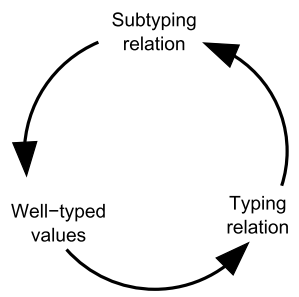
\includegraphics[width=0.4\linewidth]{images/circularity.PNG}
    \caption{Circularity in trying to define a semantic subtyping relation \citep{Castagna2005}}
    \label{fig:circ}
\end{figure}

\section{Nominal vs Structural Subtyping}
\label{sec:struct}

Orthogonally to the discussion above of syntactic versus semantic approaches, for object-oriented languages such as SFJ, there also exists two other opposing approaches to defining a subtyping relation: the \emph{nominal} and \emph{structural} approaches.

Nominal subtyping is based on explicit declarations by the developer of the class-hierarchy and is the approach used in Java.
$A$ is a subtype of $B$ if and only if it declared to be so by including an explicit declaration that $A$ extends $B$.
In Java, every user-defined class either extends another class or the root $Object$ class, creating a tree-like subtyping hierarchy.

Structural subtyping uses the structure of classes, namely its fields and methods, to define the subtyping relation.
$A$ is a subtype of $B$ if and only if the fields and methods of $B$ are a subset of the fields and methods of $A$, and if the field and method return types are covariant and the method argument types are contravariant.
This is similar to the requirements in Liskov's Substitution Principle \citep{Liskov1994} without the behavioural conditions.

\begin{equation}
    \label{eq:substitutionprinciple}
    \begin{array}{ll}
        \syndecl{Apple}{\mathit{Object}} {
         &
            \qquad
            \syndecl{Steel}{\mathit{Object}} {
                \\
                \qquad\quad \ldots \qquad
         &
                \qquad\qquad\quad \ldots
                \\
                \qquad\quad \textbf{float}\ \mathit{setPrice}\ (\textbf{int}\ a)\{\ \ldots\ \}\qquad
         &
                \qquad\qquad\quad \textbf{int}\ \mathit{quality}
                \\
            }
            \qquad\quad\qquad
         &
            \qquad\qquad\quad \textbf{int}\ \mathit{setPrice}\ (\textbf{float}\ a)\{\ \ldots\ \}
            \\
         &
            \qquad }
    \end{array}
\end{equation}

We can see in Equation \ref{eq:substitutionprinciple} that $Steel$ is a structural subtype of $Apple$, as the use of any field or method of $Apple$ would also be defined in $Steel$.
All field or method return types in $Steel$ are the same or more restrictive than those that also occur in $Apple$, and all method argument types are the same or less restrictive in $Steel$ than in $Apple$.
However, $Apple$ is not a subtype of $Steel$ as $Apple$ is missing the $quality$ field.
In other cases a pair of classes can both be subtypes of one another.

Nominal subtyping is more popular than structural subtyping, which makes it perhaps unsurprising that nominal subtyping aligns well with the syntactic approach, and structural subtyping aligns well with the semantic approach.

In our implementation of SFJ based on the work of \citet{Dardha2017, Dardha2013}, we implement a semantic type system however we include both nominal and structural subtyping.
This approach gives the programmer a choice in which approach he may wish to use, but also allows both to be used concurrently for greater flexibility and compactness in the logic a programmer may wish to implement.

\section{Featherweight Java}

The syntax of SFJ is exactly that of Featherweight Java (FJ) \citep{Igarashi1999}, with only the associated type system being different.
FJ is closely related to Java, but with a key simplification in the removal of the assignment operation.
All fields of an object cannot be changed after initialisation and all methods are pure functions.
While this restricts FJ to what is essentially a functional fragment of Java, it is still fully computationally complete.
SFJ was intentionally based on FJ instead of the full Java language because features such as concurrency and reflection are orthogonal to the purpose of demonstrating of our novel type system.

\paragraph{Multimethods}

While FJ removes some feature of the  Java language, the introduction of boolean types and semantic subtyping restores some of these.
Overloaded methods is one of these.
As suggested by \citet{Dardha2017}, we can model overloaded methods as \emph{multimethods} \citep{BC97}, which according to the authors is ``\emph{very clean and easy to understand [...] it would be the best solution for a brand new language}".
As an example \citet{Dardha2013,Dardha2017} consider the following class declarations:

\begin{equation}
    \label{multi1}
    \begin{array}{ll}
        \syndecl{A}{\mathit{Object}} {
         &
            \qquad
            \syndecl{B}{A} {
                \\
                \qquad\quad \ldots \qquad
         &
                \qquad\qquad\quad \ldots
                \\
                \qquad\quad \textbf{int}\ \mathit{length}\ (\textbf{string}\ s)\{\ \ldots\ \}\qquad
         &
                \qquad\qquad\quad \textbf{int}\ \mathit{length}\ (\textbf{int}\ n)\{\ \ldots\ \}
                \\
            }
         &
            \qquad }
    \end{array}
\end{equation}

Method \textit{length} has type $\textbf{string} \rightarrow \textbf{int}$ in $A$.
However, in $B$ it has type $(\textbf{string} \rightarrow \textbf{int}) \synwedge (\textbf{int} \rightarrow \textbf{int})$, which can be simplified as $(\textbf{string} \synvee \textbf{int}) \rightarrow \textbf{int}$.

\section{Tools}

The type system of FSJ was built using ANTLR \citep{parr2013} to define the grammar of the language and automatically create a parser for this grammar rather than having to create one by hand, which made the initial development process much quicker.
It accepts a grammar using Extended Backus-Naur Form (EBNF) \footnote{See ISO/IEC 14977 for reference, although this is not the standard used in the examples} notation to create ANTLR rules which are a list of productions or alternatives.
A general form of a rule is as follow:

\begin{equation}
    \begin{array}{llll}
        rule & : & alternative_{1}
        \\
             & | & alternative_{2}
        \\
             &   & \vdots
        \\
             & | & alternative_{n}
        \\
             & ; &
    \end{array}
\end{equation}

Each alternative production in a rule can itself be a list of elements, where an element can be another rule or a terminating token.
Since we are using EBNF notation, we can also use $*$ and $?$ to respectively signify repeated and conditional elements in a production.
We can also use $|$ to give several alternatives for a single element.
We show an excerpt taken from the SFJ grammar as an example:

\begin{equation}
    \begin{array}{llll}
        expression     & : & primExpression\ ( (PLUS | MINUS | DIV | MULT)\ primExpression)?
        \\
                       & ;
        \\
        \\
        primExpression & : & NUMBER
        \\
                       & | & TRUE
        \\
                       & ; &
        \\
        \\
        TRUE           & : & 'true'
        \\
                       & ; &
        \\
        \\
        NUMBER         & : & DIGIT\ (DIGIT)*
        \\
                       & ; &
        \\
        \\
        DIGIT          & : & '0'..'9'
        \\
                       & ; &
    \end{array}
\end{equation}

\section{Related Work}
The closest area of research would likely be the work on $\mathbb{C}$Duce
\citep{Benzaken2003}, which is also a functional language with a semantic type system designed for
working with XML documents and a continuation of the work on XDuce \citep{Hosoya2003}.
The language extended XDuce by introducing less XML specific types such as records, boolean connectives and arrow types.
This therefore makes it similar to our language in that a class-based semantic type system is a combination of the $\mathbb{C}$Duce record types with arrow types.
Muehlboeck and Tate \cite{Muehlboeck2018} define a syntactic framework with boolean connectives which has been implemented in the Ceylon programming language \citep{Ceylon2016}.

Our work and the work on $\mathbb{C}$Duce follow the functional style of $\lambda$-calculus, whereas the work by \citet{Castagna2008} extends $\pi$-calculus with semantic subtyping.
Similar work to ours creating an implementation for this would result in a Golang-like \footnote{https://golang.org/} language, creating a concurrency-focused language with more
intuitive types.
\citet{Castagna2008} found that it was required to be able to decide and resolve the atomicy, that is whether the only proper subtype is the empty type, of types in order to decide the subtyping relation, and observes that this same problem appears in $\lambda$-calculus and any other semantic-based system.
This is exactly the problem we find and solve in that we need to validate whether our type definitions are finite trees with basic types as leaves and with not cycles.

%===================================================================================================

\chapter{Syntax and Subtyping Implementation}

This chapter provides the formal syntax of the language and gives a detailed explanation of the implementation of the first core novel feature in SFJ, the semantic type system and subtyping relation.
We then consider the algorithms used in the implementation for their efficiency and any flaws the subtyping relation may have.

\section{Syntax}
\label{sec:syntax}

\subsection{Syntax of Types}

The syntax of types is given by the following grammar \citep{Dardha2013,Dardha2017}:

\begin{equation}
    \label{eq:syntaxtypes}
    \begin{array}{llll}
        \tau   & ::=                                          & \alpha \ |\ \mu
               & \mbox{\textit{Type term}}
        \\
        \alpha & ::=                                          & \zero \ |\ \btypes \ |\ [\wt{l:\tau}] \ |\ \alpha \ \bf{and}\ \alpha \ |\ \bf{not}\ \alpha
               & \mbox{\textit{Object type} ($\alpha $-type)}
        \\
        \mu    & ::=                                          & \alpha \to \alpha \ |\ \mu \ \bf{and}\ \mu \ |\ \bf{not}\ \mu
               & \mbox{\textit{Method type} ($\mu $-type)}
    \end{array}
\end{equation}

$\alpha$-types are used to type fields and $\mu$-types are used to type methods.
Type $\zero$ is the empty type.
Type $\btypes$ denotes the \emph{basic} types, such as integers, booleans, etc.
Record types $[\wt{l:\tau}]$, where $\wt l$ is a sequence of disjoint labels, are used to type objects.
Arrow types $\alpha \to \alpha$ are used to type methods.
The boolean types using ${and}$ and ${not}$ have their expected set-theoretic meanings, and ${or}$ is obtained by their combination.

\subsection{Syntax of Terms}

The syntax of terms is given by the following grammar and is based on the standard syntax of terms in FJ \cite{Igarashi1999,Dardha2013,Dardha2017}.

We assume an infinite countable set of names, with some special names: $\mathit{Object}$ indicates the root class, $\mathit{this}$  indicates the current and $\mathit{super}$ indicates the parent object.
We let  $A, B, C, \ldots$ range over classes; $a, b, \ldots$ over fields; $m, n, \ldots$ over methods and $x, y, z, \ldots$ range over variables. Constants $c$ range over an infinite countable set $\mathbb{K}$

\begin{equation}
    \label{eq:syntaxterms}
    \begin{array}{llllll}
         & \mbox{\textit{Class declaration}}  & L & \; ::= \; & \syndecl{C}{C}{\wt{\alpha \ a};\ K; \ \wt{M}\ }                         \\
         & \mbox{\textit{Constructor}}        & K & \;::=\;   & C\ (\wt{\alpha\ x})\ \{\ \synsuper(\wt{x});\ \wt{\synthis.a}=\wt{x}; \} \\
         & \mbox{\textit{Method declaration}} & M & \; ::= \; & \alpha | \mu \ m\ (\alpha | \mu \ x)\ \{\ \synret e; \}                 \\
         & \mbox{\textit{Expressions}}        & e & \; ::=\;  & x\ |\  c\ |\ e.a\ |\ e.m(e) \ | \ \synnew C(\wt{e})
    \end{array}
\end{equation}

A program $(\wt{L}, e)$ consists of a sequence of class declarations $\wt L$ and an expression $e$ to be evaluated.

A class declaration $L$ specifies the name of the class, the name of the parent class it extends, its typed fields, the constructor $K$ and its method declarations $M$.
The constructor $K$ initializes the fields of the object by assigning values to the fields inherited by the \textit{super} class and to the fields declared in the current \textit{this} class.
A method declaration $M$ specifies the signature of the method, namely the return type, the method name and the formal parameter as well as the body of the method.
Expressions $e$ include variables, constants, field accesses, method invocations and object creations.

We do not allow programs that would cause $\wt L$ to be ill-defined, such as declaring a constructor called $B$ in class $A$, multiple field or methods with the same name or declaring class $A$ which extends a non-existing type.
All these checks are also the same ones used in FJ \citep{Igarashi1999}.

In the theoretical development by \citet{Dardha2017}, unary methods are used without loss of generality: tuples of arguments can be modelled by an object that instantiates a \emph{special} class containing as fields all the needed arguments.

We include the translation of the syntax of terms into the ANTLR grammar for SFJ in Appendix \ref{lst:sfjgrammar}.

\section{Implementation of subtyping algorithm}

\subsection{Finite Types}

Since we want to use types $\tau$ in practice in SFJ, we restrict them to finite trees whose leaves are basic types with no cycles.
For example, the recursive type $A = [a : A]$ denotes an infinite program tree $\textbf{new}\ A(\textbf{new}\ A(\ \cdots\ ))$, hence we avoid it as it is uninhabitable.
Similarly the types $A = [b: B]$, $B = [a = A]$ create a cycle in our program tree and would also be impossible to inhabit.

The above type definitions are allowed but still uninhabitable in Java since you can always instantiate a object of any type by assigning the value $null$ to it.
However, since we restrict SFJ to the functional fragment of Java, we cannot do this.

Given a SFJ program, we use the ANTLR grammar, given in Appendix \ref{lst:sfjgrammar}, to create a parser and run this parser to give us an abstract syntax tree (AST) of the program.
The AST can be visited to make sure that our program is well-defined.
We mark any classes containing fields typed with only basic types as \emph{resolved} otherwise, as \emph{unresolved}.
This is then used by Algorithm \ref{alg:types}, which checks if the type definitions in the program are valid, i.e. they are finite trees whose leaves are basic types with no cycles.

\begin{algorithm}
    \caption{Algorithm which given a set of classes which are marked as resolved or unresolved, determines if all the classes can be resolved, i.e. if all the types are finite trees with no cycles and with basic types as leaves}
    \label{alg:types}

    \DontPrintSemicolon
    \KwData{$classes$, a set of classes, each marked as resolved or unresolved depending on if their fields contain only basic types.}
    \KwResult{$True$ if all classes are valid type definitions, $False$ otherwise.}
    \Begin{
        \Do{$resolutionOccured = true$}{
            $resolutionOccured \longleftarrow false$ \;
            \For{class that is unresolved in classes}{
                $resolved \longleftarrow true$ \;
                \For{field in class that contains a class type}{
                    \If{type of field is unresolved}{
                        $resolved \longleftarrow false$
                    }

                }
                \;
                \If{$resolved = true$}{
                    $class \longleftarrow resolved$ \;
                    $resolutionOccured \longleftarrow true$ \;
                }
            }
        }
        \;
        \uIf{not all classes are resolved}{
            \KwRet $False$
        }
        \Else{
            \KwRet $True$
        }
    }
\end{algorithm}

If the types in the program are finite trees whose leaves are constants with no cycles, then at each iteration of the algorithm we are going to be able to resolve at least one type or all the types are resolved.
If we do not resolve at least one type and not all types are resolved, we know we have encountered a cycle in the type definition.

\subsection{Defining the Subtyping Relation}
\label{sec:sub}

Now, given that we know that the type definitions in our program are valid, we can define the subtyping relation for this program.

Building upon the interpretation of types as sets of values, we define the subtyping relation by defining a map from a type to the set of its subtypes, with the property that the set of values of a subtype is included in the set of values of the type.
As a first step, in Equation \ref{eq:initialSubtype} we define the relation for the basic types as these will be the same for all SFJ programs and will not change.
We also define the \emph{Universe} type that holds the set of all types.

\begin{equation}
    \label{eq:initialSubtype}
    \begin{array}{llllll}
         & Double   & = \left\{Double, Float, Int, Short, Byte\right\} &  & Float & = \left\{Float, Short, Byte\right\} \\
         & Long     & =    \left\{Long, Int, Short, Byte\right\}       &  & Int   & = \left\{Int, Short, Byte\right\}   \\
         & Short    & =    \left\{Short, Byte\right\}                  &  & Byte  & = \left\{Byte\right\}               \\
         & Boolean  & =    \left\{Boolean\right\}                      &  & Void  & = \left\{Void\right\}               \\
        \\
         & Universe & = \{Double, Float, Long, Int,                                                                     \\
         &          & \quad Short, Byte, Boolean, Void\}
    \end{array}
\end{equation}

It can be seen from the initial definitions that the subtyping relation is reflexive and transitive, but not necessarily symmetric.

We would also like to note that $Int$ is not a subtype of $Float$, as in the definition of  floating-point numbers that is used in Java \footnote{See IEEE-754 for reference}, $Float$ only has 23 bits for the mantissa, meaning it cannot represent all possible values of a 32 bit $Int$ accurately and therefore $Int$ is not fully set-contained.
However, this is not the case for $Int$ and $Double$ as the latter has a 52 bit mantissa. This is also why $Long$ is not a subtype of $Double$.

\subsubsection{Final Relation}

Finally, Algorithm \ref{alg:subtyping} defines the subtyping relation for all class types.
The order in which the class types are added to the relation does not matter, as the algorithm guarantees that all subtypes for all types will be found, no matter the order. We give a description of Algorithm \ref{alg:subtyping} to aid comprehension of the algorithm.

We iterate over the keys of the relation mapping, further called the existing type.
However we can skip all those that are a basic type as no class type will have or be a subtype of a basic type.
We first check if the the class we are currently processing, further called the new type, has types in its fields or methods that are currently not in the subtyping relation.
If so, we stop and add the new type to the list of unprocessed classes, as we are not be able to correctly reason if it is a subtype due to the missing type.
This list of unprocessed classes will get recursively called to be processed again, and this process will is guaranteed to terminate because we have already checked using Algorithm \ref{alg:types} that all types are valid.

We check if the new type is a subtype of the existing type. The fields and methods of the new type must be subsets of the existing type.
We also check the structural subtyping rules for field, method return and method argument types as given in Section \ref{sec:struct}.
If these all hold, then the new type is a subtype of the existing type and is added to its relation mapping.

We then repeat the above process but instead check if the existing type is a subtype of the new type.
However we do not have to check if the call to $checkSuperSet(existingClass, class)$ return $False$ as we are guaranteed that since the existing type is already in the subtyping relation, all of its field and methods contain types that are also in the subtyping relation.
We then add the new type to its own relation mapping for reflexivity and to the \emph{Universe} type.

\begin{algorithm}
    \caption{Recursive algorithm for creating a semantic subtyping relation by calling the function \textit{generateRelation} with the set of class types that are finite trees.
        Given that we know all classes are valid types, we are guaranteed it will terminate}
    \label{alg:subtyping}

    \DontPrintSemicolon
    \KwData{
        $classes$, the set of classes in the program for which we have not yet defined a subtyping relation. \;
        $relation$, a map of types to the set of its subtypes.
        Initially the map only contains the entries defined in Equation \ref{eq:initialSubtype}. \;
    }
    \Begin{
        \Fn{generateRelation(classes: List<Class>)}{
            $unprocessed: List<Class>\ \longleftarrow []$

            \For{class in classes}{
                \If{addClass(class) = $False$}{
                    $unprocessed.add(class)$
                }
            }
            \If{$untyped \neq []$}{
                $generateRelation(unprocessed)$
            }
        }
        \;
        \Fn{addClass(class: Class) $\rightarrow$ boolean}{
            \For{existing class type in relation}{
                \If{checkSuperSet(class, existingClass) = false}{
                    \KwRet $False$\;
                }
                $checkSuperSet(existingClass, class)$\;
            }
            $relation[class].add(class)$ \;
            $relation[Universe].add(class)$ \;
            \KwRet $True$ \;
        }
        \;
        \Fn{checkSuperSet(class: Class, other: Class) $\rightarrow$ boolean}{
            $flag \longleftarrow True$ \;
            \;
            \For{field in class}{
                \If{field contains type not in relation}{
                    \KwRet $False$
                }
                \uIf{other does not contain field}{
                    $flag \longleftarrow False$
                }
                \Else{
                    \If{other.field.types does not fully contain field.types}{
                        $flag \longleftarrow False$
                    }
                }
            }
            \;
            \For{method in class}{
                \If{method contains type not in relation}{
                    \KwRet $False$
                }
                \uIf{other does not contain method}{
                    $flag \longleftarrow False$
                }
                \Else{
                    \If{other.method.types does not fully contain method.types}{
                        $flag \longleftarrow False$
                    }
                }
            }
            \;
            \If{$flag = True$}{
                $relation[other].add$
            }
        }
    }
\end{algorithm}

The subtyping algorithm finds all nominal and structural subtypes as it examines all pairs of types.
It finds all nominal subtypes as child types inherit all fields and methods of their parent class, so when considering the parent-child pair, the child is always guaranteed to be a superset.
Similarly, for all other pairs of types, the algorithm checks if one is a superset of the other, and if so, they are related by structural subtyping.
For example, in the extreme situation, the type $empty = []$, will have all classes as structural subtypes as any other class can be safely structurally substituted for it.
Therefore the same algorithm finds both nominal and structural subtypes without needing to examine the nominal subtyping hierarchy as field and method inheritance guarantees they will be found through structural subtyping.

\subsection{Typing Values and Closing the Circularity}
\label{numtypes}

Following the framework in Section \ref{sec:framework} to define a sematic type system, we next need typing rules for values, i.e. we should be able to type any expression that is able to be constructed in the syntax of terms, given in Equation\ref{eq:syntaxterms}.

\begin{equation}
    \mbox{\textit{Expressions}}        \qquad e  \; ::=\;   x\ |\  c\ |\ e.a\ |\ e.m(e) \ | \ \synnew C(\wt{e})
\end{equation}

For the expressions $e.a$ and $e.m(e)$, we can type these values simply by looking at the type of the field or return type of the method.
For object constructors $new\ C(\wt{e})$, the type of this value will be the class type $C$.
For variables $x$, we can look at what the type is of the method argument, as this is the only possible situation a variable is allowed to be used.

For the constants $c$, these are the literal values in our language such as $42$, $3.14$ or $True$.
It is not as simple as it may appear to type these correctly so that boolean type operators in our language behave correctly.

In most languages such as Java, literal values are cast to the type that is expected in the context they are used.
For example, a method $\textbf{long}\ getNum()\{return\ 42\}$ automatically casts the value to the type $long$.
In other situation such as variable type inference in Java $\textbf{var}\ x = 42$, the compiler treats the value as an $int$ too as this is the most efficient number type in hardware operations.

However, in our system, types represent sets of values which must interpret boolean connectives in a set-theoretic way.
Given the type with boolean connectives $(int\ \textbf{and not}\ byte)$, this type represents the values $-2^31$ to $2^31 - 1$ from which are removed the values $-128$ to $127$.
If we were to type the value $42$ as an integer, this would be accepted by the boolean type, but would not be in the set of values of the type, thus breaking our semantic type system.

Therefore, for all constants $c$, we use a strong typing to assign values the most restrictive types possible, i.e. the type with the smallest amount of values which still contains this value.

With this typing rule, the value $42$ is assigned the type $Byte$, so would correctly not be accepted as a value of the type $(int\ \textbf{and not}\ byte)$.

We have now defined how to type any expression that can be formed by the syntax and so have defined our typing rules.
The relation defined by the typing rules and the abstract model defined in Section \ref{sec:sub} coincide, so we have closed the circularity and defined our semantic type system.

\section{Analysis of the Subtyping Relation}

\subsection{Complexity and Efficiency of the Subtyping Algorithm}

The complexity of Algorithm \ref{alg:subtyping} is $\mathcal{O}(n)$, however the complexity of Algorithm \ref{alg:subtyping} is $\mathcal{O}(n^{2})$.
For the small example programs that SFJ has currently compiled for this has not been an issue, however if the language was extended with a standard library with several hundred if not thousand of classes, then each additional class will incur larger penalties in compiler performance.
However, the real-life impact of such a situation has not yet been explored.

Due to the fact that our subtyping relation can possibly be symmetric because of our inclusion of structural subtyping, this $n^{2}$ behaviour is needed to ensure we fully find all subtypes for each type.
In a system with solely nominal subtyping, we only need to traverse the subtype hierarchy to find all subtypes, which is a linear operation.

\subsection{Flaws of Structural Subtyping}
\label{sec:flaws}

Given the observed flaws in complexity in Algorithm \ref{alg:subtyping} due to structural subtyping, we would like to point out another flaw the reader might see in the structural approach but we argue for why we disagree with this flaw.

Consider two structurally equivalent class types $coordinate = [x:int, y:int, z:int]$ and $colour = [x:int, y:int, z:int]$.
They are structural subtypes so they can be used interchangeably in our type system, but their \emph{meaning} is completely different.
Therefore, we lose some safety in our language as it is unlikely we would like to use a colour where we expect a coordinate, but in the eyes of the type-checker, it is correct.

\citet{Dardha2017} suggest a possible extension to the language by including a $nominal$ keyword that can be used in the class signature to indicate that this class should only be considered by the nominal component of the type system.
However, being optional, we argue that this would create more bugs than problems it would solve due to forgetting the keyword.
A similar issue occurs for example with destructors in C++ classes. Leaving out the virtual keyword of the parent class destructor in certain situations can lead to memory leaks.
We therefore argue instead that an additional \emph{structural} keyword could be introduced as an extension to the language which specifies that this class can have structural subtypes.
However, a class with this keyword is not added to the subtyping relation of other structurally similar classes which are not marked \emph{structural} as this would weaken the invariant conditions of this class.

In languages with solely nominal subtyping such as Java, one can define an overridden method to perform the opposite logic to what the super class is expecting, such as:

\begin{equation}
    \begin{array}{ll}
        \syndecl{A}{\mathit{Object}} {
         &
            \qquad
            \syndecl{B}{A} {
                \\
                \qquad\quad \ldots \qquad
         &
                \qquad\qquad\quad \ldots
                \\
                \qquad\quad \textbf{int}\ length\qquad
         &
                \qquad\qquad\quad \textbf{int}\ getLength()\{\ \synret{-length}\ \}
                \\
                \qquad\quad \textbf{int}\ getLength()\{\ \synret{length}\ \}\qquad
         &
                \qquad}
            \\   }
    \end{array}
\end{equation}

Therefore, even languages without structural subtyping leave an expectation on the developer to check what they are doing is correct.
Hence we argue that the integration of both in SFJ is a valid idea as either subtyping system is no more or no less than the other, so having both available gives the user the choice to use either to where they are best suited, which should lead to more correctly defined abstractions in the program, which should lead to less bugs in the program.

For example, when structural subtyping is used correctly, it makes certain recurring challenging programming tasks effortless.
Take the task of dependency injection in testing for mocking class behaviour.
In languages like C++, we may wish to not make the methods in our classes virtual (making them not overridable) to perhaps not incur the performance overhead of virtual methods.
In these situations, mocking such a class is near impossible without changing the type hierarchy or class definition.
With structural subtyping, we simply define a class with the same fields and method signatures, and can provide our own implementations in the methods.
Because the type will be structurally similar, it is effortless to use our new class as an argument where the old class is expected.

\chapter{Exploiting Semantic Subtyping}

In this chapter we demonstrate that having defined the mathematical machinery behind the semantic type system, it is easy to add features into the language which exploit the set-theoretic subtyping system and make writing SFJ programs more concise and intuitive.
This introduces the second core novel addition in SFJ of boolean types, along with method types and multi-methods.

\section{Implementation of Boolean Types}
\label{sec:bool}

Now that we have define our semantic type system, it is easy to implement boolean types in our language.

\subsection{Illustrative example of Boolean Types}

We demonstrate the implementation of boolean types by using our main motivational example given by \citet{Dardha2013} which illustrates the benefits of boolean types.

\subsubsection{The Polygons}

Our example considers a set of polygons, such as triangles, squares and rhombuses.
We want to define a method \emph{diagonal} that takes a polygon and returns the length of its longest diagonal, however such a method only is defined for polygons that have at least four sides
Therefore we need to find a way of implementing the type hierarchy in such a way that triangles are excluded.
In Java this could be done in the following way:

\begin{equation}
    \begin{array}{l}
        \synclass Polygon \ \{ \ldots\}
        \\
        \syndecl{Triangle}{Polygon} {\ldots}
        \\
        \syndecl{Other\_Polygons}{Polygon} {
            \\
            \qquad \ldots
            \\
            \qquad \textbf{double}\ diagonal(Other\_Polygons \ shape)\ \{\ldots \}
            \\
        }
        \\
        \syndecl{Square}{Other\_Polygons}{\ldots}
        \\
        \syndecl{Rhombus}{Other\_Polygons} {\ldots}
    \end{array}
\end{equation}

Or by means of an interface \emph{Diagonal}:

\begin{equation}
    \label{eq:interface}
    \begin{array}{l}
        public \ \syninterface Diagonal\ \{
        \\
        \qquad \textbf{double}\ diagonal(Polygon \ shape);
        \\
        \}
        \\
        \synclass Polygon \ \{\ldots\}
        \\
        \syndecl{Triangle}{Polygon} {\ldots}
        \\
        \synidecl{Square}{Polygon} \synimpl Diagonal \ \{\ldots\}
        \\
        \synidecl{Rhombus}{Polygon} \synimpl Diagonal \ \{\ldots\}
        \\
        \hspace{4.5cm} \ldots
    \end{array}
\end{equation}

However, the first is error-prone and could be said to be not self-documenting \citep{schach2007}, i.e. the type hierarchy does not explain why this extra class $Other_Polygons$ has been created.
The second solution is more informative, however given many other methods we may want wish implement, it would quickly become cumbersome to have a long list of interfaces for each polygon we add.

If we were not able to write our own abstractions and rather were given a legacy system, the most likely and natural abstraction would be for \emph{Polygon} to be the parent type and all more specific shapes extend this class.
Now the only way we would be able to define such a method \emph{diagonal} is to use \emph{instanceof} to see the type of the argument $Polygon$ at run-time and throw an error if we encounter a triangle.
However now we no longer check at compile-time whether the arguments we are passing are correct, leading to possible bugs at run-time.

In SFJ, we instead propose a more elegant solution with the use of boolean types where the check for excluding triangles happens at compile-time.
We can simply define a method \emph{diagonal} which takes an argument of type \emph{Polygon} \textbf{and not} \emph{Triangle}.

\begin{equation}
    \label{eq:polygons}
    \begin{array}{l}
        \synclass Polygon \ \{\ldots\}
        \\
        \syndecl{Triangle}{Polygon} {\ldots}
        \\
        \syndecl{Square}{Polygon} {\ldots}
        \\
        \syndecl{Rhombus}{Polygon} {\ldots}
        \\
        \synclass Diagonal \ \{
        \\
        \qquad \ldots \\
        \qquad \textbf{double}\ diagonal((Polygon\ \textbf{and not}\ Triangle) \ shape)\{\ldots\}
        \\
        \}
    \end{array}
\end{equation}

\subsection{Type-Checking Boolean Types}
\label{typecheck}

\begin{equation}
    \label{eq:initialSubtype}
    \begin{array}{llllll}
         & Double   & = \left\{Double, Float, Int, Short, Byte\right\}     &  & Float    & = \left\{Float, Short, Byte\right\} \\
         & Long     & =    \left\{Long, Int, Short, Byte\right\}           &  & Int      & = \left\{Int, Short, Byte\right\}   \\
         & Short    & =    \left\{Short, Byte\right\}                      &  & Byte     & = \left\{Byte\right\}               \\
         & Boolean  & =    \left\{Boolean\right\}                          &  & Void     & = \left\{Void\right\}               \\
         & Polygon  & = \left\{Polygon, Triangle, Square, Rhombus \right\} &  & Triangle & = \left\{Triangle\right\}           \\
         & Square   & = \left\{Square\right\}                              &  & Rhombus  & = \left\{Rhombus\right\}            \\
         & Diagonal & = \left\{Diagonal\right\}
        \\
        \\
         & Universe & = \{Double, Float, Long, Int, Short, Byte                                                                \\
         &          & \quad Boolean, Void, Polygon, Square                                                                     \\
         &          & \quad Square, Rhombus, Diagonal\}
    \end{array}
\end{equation}

We first generate the subtyping relation for our solution in Equation \ref{eq:polygons} to give the relation in Equation \ref{eq:initialSubtype}.

Recall the method \emph{diagonal} in class \emph{Diagonal}, we can see that the result of the set operation on its parameter type gives the following set of polygons:

\begin{equation}
    \label{eq:polygonsandnottriangle}
    Polygon\ \textbf{and not}\ Triangle = \left\{Polygon, Square, Rhombus \right\}
\end{equation}

The \emph{\textbf{not} Triangle} operation is achieved by $Universe \setminus Triangle$.
Therefore if we type-check the following SFJ expression:

\begin{equation}
    (\textbf{new}\ Diagonal()).diagonal(\textbf{new}\ Square())
\end{equation}

the argument $new\ Square()$ is typed using our typing rules given in Section \ref{numtypes} to be of type $Square$, and the subtypes of Square is $\{ Square \}$ which is fully contained in the set of the parameter type $\left\{Polygon, Square, Rhombus \right\}$, so this expression successfully type-checks.

On the other hand, given the expression:

\begin{equation}
    (\textbf{new}\ Diagonal()).diagonal(\textbf{new}\ Triangle())
\end{equation}

the subtypes of the argument is $\{ Triangle \}$ which is not contained in the set of subtypes for the parameter so therefore this does not type check.

We can also demonstrate the example from Section \ref{numtypes}. Recall the type $(int\ \textbf{and not}\ byte)$. The result of the set operations would be:

\begin{equation}
    \label{eq:intnotbyte}
    int\ \textbf{and not}\ byte = \left\{Int,\ Byte\right\}
\end{equation}

Then given the classes:

\begin{equation}
    \begin{array}{l}
        \synclass{Integer} \ \{
        \\
        \qquad \ldots
        \\
        \qquad \textbf{int}\ num
        \\
        \qquad \textbf{int}\ getNum()\{return\ this.num\}
        \\
        \}
        \\
        \synclass{Calculator}\ \{
        \\
        \qquad \ldots \\
        \qquad \textbf{double}\ acceptLargeNum((int \textbf{ and not } byte) \ n)\{\ldots\}
        \\
        \}
    \end{array}
\end{equation}

with the following expression to evaluate:

\begin{equation}
    (\textbf{new}\ Calculator()).acceptLargeNum((\textbf{new}\ Integer(2)).getNum())
\end{equation}

we can show that this expression does not type-check.
The value $2$ is given the type $Byte$, but is valid for the field \emph{num} as the subtypes of $Byte$, namely just itself, is fully contained in the set of subtypes of $Int$.
However, the argument to the function $acceptLargeNum$ is of type $Int$, which has subtypes $\{Int, Short, Byte\}$.
We can see that this is not fully set-contained in the set of subtypes of Equation \ref{eq:intnotbyte}, so the expression does not type-check.

\subsection{How Boolean Types are Represented in SFJ}

We next show how we ensure that compound boolean statements are evaluated consistently and how we represent the boolean types in our implementation.

If we refer to the SFJ grammar in Appendix \ref{lst:sfjgrammar}, we can see in the \emph{type} production rule we enforce that every single boolean connective is surrounded by brackets to enforce consistency in the definitions.
Take the boolean type $type_{1} \textbf{ and } type_{2} \textbf{ or } type_{3}$.
Without brackets, we do not know how to consistently evaluate this type as they could mean different things:

\begin{equation}
    \begin{array}{llll}
        type_{1} \textbf{ and } (type_{2} \textbf{ or } type_{3}) & =  & (type_{1} \textbf{ and } type_{2}) \textbf{ or } (type_{1}\ \textbf{and} \ type_{3})
        \\
                                                                  & or &
        \\
        (type_{1} \textbf{ and } type_{2}) \textbf{ or } type_{3} & =  & (type_{1} \textbf{ or } type_{2}) \textbf{ and } (type_{1}\ \textbf{or} \ type_{3})
    \end{array}
\end{equation}

Therefore such a type is not allowed and the user has to specify which of the two alternatives they mean to use.

Secondly, once we have a boolean type which is consistent, we can evaluate the final result by storing it as a tree, such as shown in Figure \ref{fig:boolfig}.
Starting from the root node, we check if it is a type or a boolean connective.
If it's a type, we can look up the type in our subtyping relation and return the set of of its subtypes.
However, if its a boolean connective, we know it will have two child nodes and we can inspect them  and apply the same process until they both return us a set of subtypes.
We can then get the result of the boolean connective node by applying the corresponding set operation to the two sets of subtypes it received.

\begin{figure}
    \label{fig:boolfig}
    \centering
    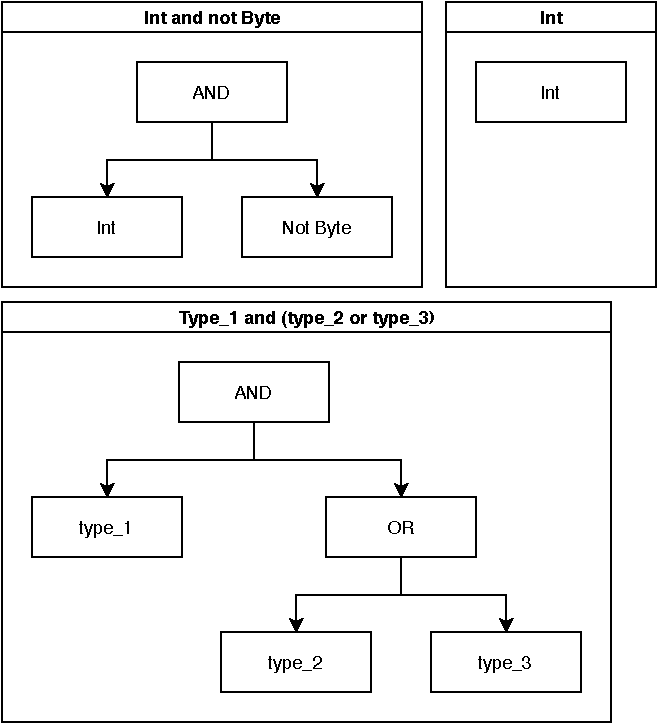
\includegraphics[width=0.7\linewidth]{images/diag.pdf}
    \caption{Representation of how the types $int$, $int \ \textbf{and not}\ byte$ and $type_{1}\ \textbf{and}\ (type_{2}\ \textbf{or}\ type_{3})$ are stored.}
\end{figure}

\section{Unusable Boolean Types}
\label{unusable}

Similar to structural subtyping, we would like to highlight a potential issue the reader might notice with the use of boolean types.

The use of boolean types can restrict the set of subtypes we accept, such as with the example of $Polygon \textbf{ and not } Triangle$ in Equation \ref{eq:polygonsandnottriangle}.
However, a problem arises in that we can widen the set of subtypes that we accept such that there is no guarantee about how the object can be used at run-time.

Take the subtype relation from the Polygons example, Equation \ref{eq:initialSubtype}.
If we create a boolean type $\textbf{not}\ Byte$, this corresponds to the set of accepted subtypes $\{Short, Int, Long, Float, Double, Boolean, \allowbreak Void, Polygon, Square, Rhombus, Triangle\}$.
An argument of such a type accepts many values, but what can such an argument actually be used for?

It is not guaranteed that it is a numerical value that can be used in a mathematical expression, nor is it guaranteed to be a polygon object whose field or method we can access.
If we were to try and access a field, then at runtime this would sometimes be correct but in other times this would cause an error.
So in which ways should such a type be allowed to be used in expressions?

We follow the opinion we expressed in Section \ref{sec:flaws} and leave an expectation on the developer to use boolean types in such a way that they are useful.
We implement the simple check that in use of a value that has a boolean type, then at least one of the subtype alternatives is valid, e.g. the field we are trying to access is defined for at least one subtype. However otherwise leave the developer to check that the type is used correctly.

An alternative would be strict checking that the use of a value is defined for all of its subtypes. The \emph{diagonal} method from the Polygons example \ref{eq:polygons} would still be an accepted type, however almost any use of the $\textbf{not}\ Byte$ type would result in a compiler error.

However we feel this would go against our aims of creating a language where the programmer is given the choice to use a more expressive type system.
Additionally, a static type checking tool could be developed for SFJ which warns the user if a value is used in a way which is not defined for all of its subtypes, giving the user greater confidence in using boolean types.

\section{Method Types}

While our more elegant solution to the Polygons problem \ref{eq:polygons} is an improvement in terms of compactness and clarity, it is not perfect.
One oversight of this solution is that we define a single method for all accepted alternatives, however the implementation of calculating the longest diagonal will be different for each of them.
To solve this using the language constructs available to us would again involve us having to use \emph{instanceof} to check the type at run-time and executing the correct implementation for each type.
Alternatively we could also have the following implementation:

\begin{equation}
    \begin{array}{l}
        \synclass Polygon \ \{
        \\
        \qquad \ldots
        \\ \qquad \textbf{double}\ diagonal()\{\ldots\} \\ \}
        \\
        \syndecl{Triangle}{Polygon} {\ldots}
        \\
        \syndecl{Square}{Polygon} {
            \\
            \qquad \ldots

            \\ \qquad \textbf{double}\ diagonal()\{\ldots\} \\ }
        \\
        \syndecl{Rhombus}{Polygon} {
            \\
            \qquad \ldots

            \\ \qquad \textbf{double}\ diagonal()\{\ldots\} \\ }
        \\
        \\
        \synclass Diagonal \ \{
        \\
        \qquad \ldots \\
        \qquad \textbf{double}\ diagonal((Polygon\ \textbf{and not}\ Triangle) \ shape)\{\synret\ shape.diagonal()\}
        \\
        \}
    \end{array}
\end{equation}

However what if the class \emph{Polygon} also did not implement the method diagonal, seeing how it is a generic class and we do not how we would be able to calculate a diagonal for it.
The type declaration that is currently used in the method \emph{diagonal} would no longer be valid and we instead would have to specify each alternative manually $(Square\ \textbf{or}\ Rhombus\ \textbf{or}\ \ldots)$ which is tedious and error-prone.

This is where the arrow type (method type) from our syntax of types \ref{eq:syntaxtypes} can be used. We can instead define the class \emph{Diagonal} as follows:

\begin{equation}
    \begin{array}{l}
        \synclass Diagonal \ \{
        \\
        \qquad \ldots \\
        \qquad \textbf{double}\ diagonal((diagonal: \textbf{Void} \rightarrow \textbf{Double})\ shape)\{\synret\ shape.diagonal()\}
        \\
        \}
    \end{array}
\end{equation}

We define the type as accepting any type and its subtypes which implement a method called \emph{diagonal} which is a method from the type \emph{Void} to a \emph{Double}.
We also finally see that the type \emph{Void} is used in SFJ to indicate a method that has no arguments, as due to being a functional language, we do not have any fields or method return types which can be of type \emph{Void}.

In order to type-check the value passed to such an argument, we can at compile-time build a collection of types $\{type_{1},\ type_{2},\ \ldots\}$ which have this method.
We can do this the simply iterating over the same list of classes in the program as when we were creating our subtyping relation and checking for the presence of the required method.
The set of accepted types would then be the union of all their corresponding subtypes $([\![type_{1}]\!]_{B} \cup [\![type_{2}]\!]_{B} \cup\ \ldots)$.

However, calculating this collection of types for each method of every class would be computationally unnecessary as only few of these would be used for method types.
Therefore we only compute on demand during type-checking them when we come across such a type.
This makes compilation times exceedingly quicker the more classes are in our program, especially if we cache the method types we have already encountered, as it is likely to come up again if it has already been used once.
However, this caching behaviour has currently not been implemented in SFJ as compilation speed has so far been orthogonal to the aims of this project.

We can therefore use method types to statically include or exclude a portion of our type hierarchy.
However unlike the use of interfaces such as in the suggested Java solution \ref{eq:interface} to the Polygons problem, the values that can be accepted by a method type do not have to be related to each other in any way in the class hierarchy.
This becomes increasingly useful if we have a legacy system as we can still accept all the classes that have defined \emph{Diagonal} methods without having to go back and add interface implementations.

\section{Multi-methods}

One key feature that we restore in SFJ that we lost from Java is that of overloaded methods, however we implement these as multi-methods.
Methods within a class must still have unique names, however when using nominal subtyping, we can extend the inherited method.

For example, looking back at Equation \ref{multi1}, the method \emph{length} has type $\mathbf{string} \rightarrow \mathbf{int}$ in $A$.
However, in $B$ it has type $(\textbf{string} \rightarrow \textbf{int}) \synwedge (\textbf{int} \rightarrow \textbf{int})$,
which can be simplified as $(\textbf{string} \synvee \textbf{int}) \rightarrow \textbf{int}$.

However, what happens if the extended input types are not disjoint, unlike the example in Equation \ref{multi1}:

\begin{equation}
    \label{multi}
    \begin{array}{ll}
        \syndecl{A}{\mathit{Object}} {
         &
            \qquad
            \syndecl{B}{A} {
                \\
                \qquad\quad \ldots \qquad
         &
                \qquad\qquad\quad \ldots \
                \\
                \qquad\quad \textbf{float}\ \mathit{length}\ (\textbf{float}\ n)\{\ \ldots\ \}\qquad
         &
                \qquad\qquad\quad \textbf{int}\ \mathit{length}\ (\textbf{int}\ n)\{\ \ldots\ \}
                \\
            }
         &
            \qquad }
    \end{array}
\end{equation}

Considering the example in Equation \ref{multi}, if we called method \emph{length} on an object of class \emph{B} with the value $2$, should it perform the expression in its own method or the method of $A$ considering they both accept it as an argument.
No matter which one we choose, the return type of the value is still going to be the same $\textbf{float}\ \synvee\ \textbf{int}$ which simplifies to $\textbf{float}$, however the expressions in the methods could be entirely different.

We decided to follow common object-oriented conventions and we perform the expression of the multi-method that is closest to the class of the object we are calling it on, i.e. in the case of our example, the method \emph{length} in $B$ would be called.

We do this storing the type of \emph{length} in $B$ without regard of multi-methods, as we can always generate the return type by walking up the tree of parent types, but it allows us to decide which implementation to choose.

\section{Additional Features}

One of the features that we implemented to increase the usability of SFJ as a language is removing the need for forward declarations of classes.
This means that classes can be can be used before they are defined later on in the file of the program, such as in Java.

For example for our polygons example \ref{eq:polygons} this is not necessarily obvious, but it could have been also defined as follows:

\begin{equation}
    \begin{array}{l}
        \synclass Diagonal \ \{
        \\
        \qquad \ldots \\
        \qquad \textbf{double}\ diagonal((\textit{Polygon} \textbf{ and not }  \textit{Triangle}) \ shape)\{\ldots\}
        \\
        \}
        \\
        \synclass Polygon \ \{\ldots\}
        \\
        \syndecl{Triangle}{Polygon} {\ldots}
        \\
        \vdots
    \end{array}
\end{equation}

In a language like C++, this would have required defining the structure of all the classes in a header file, however by incorporating it into the language, we make the language easier to use.

Implementing this requires that we do multiple passes over the AST of our program, which will cause an impact on compilation speed.
On our first pass of the AST we gather all the signatures of the classes and their field and methods and store it in a program tree, which is a condensed version of the AST with all unneeded information removed. At this point we have all the information needed to create the subtyping relation by running Algorithm \ref{alg:subtyping} and Algorithm\ref{alg:subtyping} on the all the class nodes at the top of our program tree.

We can now do a second pass over our program, this time on our program tree.
During this pass we check what we were unable on our first pass such as checking that the arguments given to the \emph{super} call inside class constructors type-check with respect to the subtyping relation.
Now that we have our typing rules and subtyping relation, we can now also make sure that the expressions in methods type-check according to their expected return type.


\chapter{Code Generation}

In this chapter, we define for code generation for a SFJ program as just a type system which we can use to type-check programs is without much use if we cannot run these programs on a computer.

\section{Implementation}

Due to extenuating circumstances around the COVID-19 pandemic, the code generation implementation of SFJ was not able to be completed in this project, however we still provide the theoretical implementation for the use of any future work.

Given the similarity of SFJ to Java, we felt that the usage of the Java Virtual Machine (JVM) \footnote{See https://docs.oracle.com/javase/specs/jvms/se7/html/ for reference} would be most suitable for code generation by transpiling SFJ programs into Java bytecode.
This is the approach used by object-oriented languages such as Kotlin \footnote{https://kotlinlang.org/} and many others.

The key challenge in implementing code generation compared to other languages which transpile their programs into bytecode is that for example, a single field in SFJ with type $int\ or\ bool$ actually represents two Java fields, one of type $int$ and another of type $bool$, of which only one is inhabited with a value.

Therefore to reduce the amount of alternatives for which we would need to generate code, we first analyse our program and reduce the boolean types by keeping only the alternatives which actually get used in the program.
For example, if the field of type $int\ or\ bool$ only ever gets initialised with a boolean value, we can reduce it and make it a field of a single type $bool$.
Similarly the numerical basic types can also be reduced to their largest type without consequence, such as $int\ \textbf{and not}\ byte$ can be reduced to just $int$ as we have already type checked all literal values passed to such a type.

After reducing the boolean types in our program, we have to expand all our still existing boolean types and consider each alternative in the result of the set operation.
Staying with the example of a field named $f1$ of type $int\ or\ bool$, we would define in our class two fields $int\_f1$ and $bool\_f1$ with types $int$ and $boolean$ respectively.
In order to initialise these field, we use the constructor overloading capabilities of Java to generate an overloaded version for all combinations of constructor parameters.
In each constructor, each expanded parameter alternative that is not used is initialised to $null$ and only the expanded parameter that matches the type of the parameter in this constructor is initialised with a value.

For methods, we also use the overloading capabilities of Java to define a method for each type in the expanded method parameter, all with the same method body.
Depending on which alternative the argument inhabits at run-time, a different method will be dispatched to.
Then depending on if the actual argument is valid for the method body, the method will return a value or we will encounter an exception from the JVM.

For the access of any field of an object, we generate code that checks for each alternative of the field if it is non-null and if it is non-null, then we perform the generated code for the remaining expression. However at runtime, only one branch of will be true, and this is the branch of generated code which will be executed.

For structural subtypes, we create an actual nominal subtype with the same implementation for each structural subtype a type has, so that it is accepted as a proper subtype in Java.

Like methods with boolean types, we implement methods with method types the same way by defining an overloaded alternative for each type that implements the method of the method type.

We have now defined the code generation for each expression in our syntax of terms and for field, constructor and method declarations, so therefore have defined how to generate the bytecode for any SFJ program.

\section{Problems with Code Generation}

One of the problems that can easily be seen is that when the boolean types are used incorrectly such as the example $\textbf{not}\ Byte$ from Section \ref{unusable}, then we will generate lots of bytecode as we have to consider each alternative.
While this should theoretically not affect the time for the bytecode to run on the JVM, the time for the compiler to generate bytecode for each alternative could take a significant amount of time, especially when more and more classes are added to the program.
However, it would have to be evaluated if compilation times would be affected so much that compilation is infeasible for large programs.
Yet, considering that there exist project with multi-million lines of Java code \footnote{https://www.visualcapitalist.com/millions-lines-of-code/, accessed 31/03/2020} which compile in an acceptable amount of time, we do not think this should be a problem for most programs.

%===================================================================================================

\chapter{Evaluation}

This chapter describes the evaluation methods for this project.
The quality of the language as a software product was tested.
The quality if the language in terms of ease of use of new users was also evaluated.
Finally, the language was evaluated if it met all the requirements that we set of the type of programming problems it should have made easier.

\section{Testing}

One of the major limitations we found of testing a programming language which was built as non-commercial, prototype product is that code ends up very tightly coupled, which makes unit testing difficult.
Therefore it was decided that the code was mainly tested using regression testing of a single constantly evolving test program which aimed to cover all possible edge cases of class definitions.
However, another difficulty which was found is that due to the infinite possibilities of programs, it is much more difficult to find edge cases.
When your input is simpler such as integers, there are well known edge cases such as zero, one, negative one, and the max values.

The regression test was used to create a code coverage report, pictured in Figure \ref{fig:coverage}. The testing achieves a line coverage of 71\%, which is close to the 80\% figure that is aimed for in software project by companies such as Microsoft \footnote{https://docs.microsoft.com/en-us/visualstudio/test/using-code-coverage-to-determine-how-much-code-is-being-tested}

\begin{figure}[H]
    \label{fig:coverage}
    \centering
    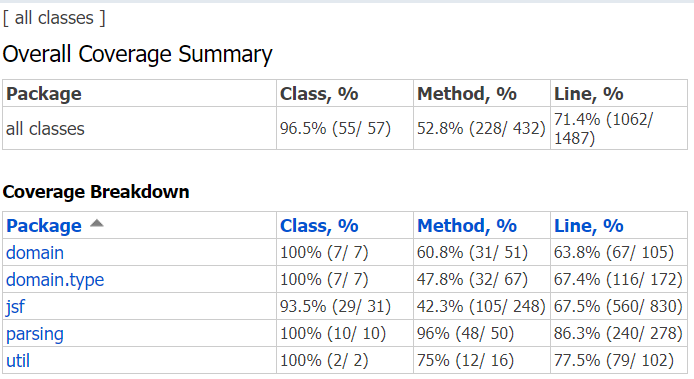
\includegraphics[width=0.7\linewidth]{images/coverage.png}
    \caption{Coverage Report indicating a line coverage of 71\%}
\end{figure}

\section{User Evaluation}

The second evaluation metric of the language was to evaluate whether users found the semantic type system and boolean types obvious to use, however due to extenuating circumstances this could not be conducted.
We include our evaluation plan as an area of future work.

\subsection{Evaluation Strategy}

Users are to be given the following scenario:

``
Our problem considers a set of polygons, such as triangles, squares and rhombuses.
We want to define a method \emph{diagonal} in a class \emph{Diagonal} that takes a polygon and returns the length of its longest diagonal, however such a method only is defined for polygons that have at least four sides.
Therefore we need to find a way of implementing this method in such a way that triangles are excluded.

You are required to define at least the following four classes: Triangle, Square and Rhombus and Diagonal.
The class Diagonal must have a single method \emph{diagonal} that upon being passed an object of type Square or Rhombus, returns the integer two.
Upon being passed an object of type Triangle, it raises any sort of exception, whether it be at compile-time or run-time.
The classes Triangle, Square, Rhombus and Diagonal are not required to have any fields.
You do not have to run the program to complete the task but can do so if wanted.
''

and are given one minute to read it.
They are required to write a solution to the scenario in Java on a Windows machine using the program Notepad without any assistance of other people or programs.
They are timed and monitored for how long it takes them to create a solution.

The same participants are then repeat this but implement the solution in SFJ.
All are given Section \ref{sec:syntax} as documentation to the language.
Half of the participants are also given the additional documentation as follows:

``
The interpretation of types is of sets of values, so we define the subtyping relation by defining a map from a type to the set of its subtypes, with the property that the set of values of a subtype is included in the set of values of the type.

\begin{equation*}
    \begin{array}{l}
        Int = \{Int, Short, Byte\}
        \\
        Byte = \{Byte\}
        \\
        int \textbf{ and not } byte = \left\{Int,\ Short\right\}
    \end{array}
\end{equation*}
''

The participants shall all be students who are enrolled on a single or joint honours Computer Science degree of any year of study.
The time to solve both problems shall be anonymised, but their year of study and programming language of choice shall be recorded for analysis purposes.

The aim of the experiment is that being given the problem and being allowed to think it through in Java beforehand, then when given the second problem, the participants who are not given the additional documentation perform the same task in the same or longer time, whereas the participants who are given the additional documentation perform the task quicker than their first time.
It shows that when given an unrelated example of the semantic type system and boolean types, users can apply it to the problem given to them, showing that the language is intuitive to use.

\section{Summary}

One of the main requirements of SFJ was that it made programming more intuitive and therefore reduced the number of lines needed for the same problem.
We can see from Listings \ref{lst:polygonsjava} and \ref{lst:polygonsfj} that the solution in SFJ took only thirteen lines whilst the equivalent solution in Java took sixteen lines of code.
While we do not have such a comparison for a program of larger length and complexity, it is already visible that if we restrict Java to an equivalent functional subset as SFJ, then we are able to express all functional Java programs in SFJ, meaning that we can only make our programs more concise.

\begin{lstlisting}[language=Java, caption={Polygons example solution in Java}, label=lst:polygonsjava]
    interface Diagonal {
        double diagonal(Polygon shape);
    }
    class Polygon {
        Polygon(){}
    }
    class Square extends Polygon implements Diagonal {
        Square(){}
        double diagonal(){return 2;}
    }
    class Triangle extends Polygon {
        Triangle(){}
    }
    class DiagonalCalculator {
        double getDiagonal(Diagonal shape){return shape.diagonal();}
    }
\end{lstlisting}

\begin{lstlisting}[language=Java, caption={Polygons example solution in SFJ}, label=lst:polygonsfj]
    class Polygon {
        Polygon(){}
    }
    class Square extends Polygon {
        Square(){}
        double diagonal(){return 2;}
    }
    class Triangle extends Polygon {
        Triangle(){}
    }
    class DiagonalCalculator {
        double diagonal((Polygon and not Triangle) shape){return shape.diagonal();}
    }
\end{lstlisting}

The language satisfies our minimum requirements of a semantic type system which represents type as sets of values, and complements this type system with boolean types, as shown in Section \ref{sec:bool}.

We can also see how expressive the end language is by seeing if we are able to reintroduce the typical programming constructs that were removed in FJ given by \citet{Dardha2017} Section 8.3.

Our current implementation of multi-methods is able to reintroduce the \emph{instanceof} construct, exactly as defined.
However for the implementation of the \emph{if-then-else}, we are missing the ability to use singleton values from our types of sets of values as parameter types, such as the $[\textbf{true}]$ type. If we did have this construct, we would also be able to add the \emph{try-catch} construct back into our language.
It is visible however how the mathematical model is still more powerful than our language due to the much greater flexibility it has, but our language is close and has implemented other additional features such as method types.

As a software project, the language could be improved by the introduction of a formal testing suite with targeted unit tests.
However what would be better is to expand the current regression testing even more.
Given that the regression tests are testing a compiler, they also automatically show which feature in our language has regressed by the error message of the compiler.

%===================================================================================================

\chapter{Demonstration Paper}

This chapter briefly describes the tool paper about SFJ which was submitted to COORDINATION 2020.
We include a reference to the paper and demonstration video that were submitted \citep{UD20}.

\section{COORDINATION 2020}

The 22nd International Conference on Coordination Models and Languages (COORDINATION) is a conference which aims to promote research into new models, architectures, languages and verification techniques in order to cope with the complexity induced by the demands of modern software development.
A paper was submitted as a tool paper to demonstrate our innovative prototype language which through semantic subtyping and boolean types, allows users to define more intuitive types which should lead to fewer logical bugs in programs.
The paper is titled \emph{SFJ: An implementation of Semantic Featherweight Java} and discusses a subset of this dissertation in less detail.
As of the time of writing, the acceptance of the paper is still pending.
The abstract is as follows:

\begin{adjustwidth}{50pt}{50pt}
    Subtyping is a key notion in programming languages, as it allows more flexibility in coding.
    There are two approaches to defining subtyping relations: the \emph{syntactic} and the \emph{semantic} approach.
    In semantic subtyping, one defines a model of the language and an interpretation of types as subsets of this model.
    Subtyping is defined as inclusion of subsets denoting types.
    An orthogonal subtyping question, typical of object-oriented languages, is the \emph{nominal} vs. \emph{structural} subtyping.
    Dardha \emph{et al.} \cite{Dardha2013,Dardha2017} defined boolean types and semantic subtyping for Featherweight Java (FJ) and integrated both structural and nominal subtyping, thus exploiting the benefits of both approaches.
    However, these benefits were illustrated only at a theoretical level, but not exploited practically.

    In this paper, we present SFJ---Semantic Featherweight Java, an implementation of FJ which features boolean types and structural subtyping as well as nominal subtyping.
    The benefits of SFJ, illustrated in the paper and the video (with audio/subtitles) \cite{UD20}, show how static typechecking of boolean types and semantic subtyping gives higher guarantees of program correctness, more flexibility and compactness of program writing.
\end{adjustwidth}


%===================================================================================================

\chapter{Conclusion}

This paper has discussed the reason why type systems exist, and the motivation for why we should research more expressive type systems.
We incorporate a semantic type system as an extension to Featherweight Java and present this as Semantic Featherweight Java.
The syntax and implementation of SFJ and its semantic subtyping relation were explained in depth, before we exploited it to easily implement boolean types.
This chapter provides a full summary of the paper and project and looks at what future work remains to be done on this project and on type systems.

\section{Summary}

In summary, a semantic type system is one where types represent subsets of values in the model of our language.
The subtyping relation is then defined as inclusion of sets denoting types.
We extend Featherweight Java with such a type system to present Semantic Featherweight Java.
SFJ has an extended type algebra with boolean connectives: \emph{and}, \emph{or} and \emph{not} which behave according to their expected set-theoretic interpretation.
SFJ also gives the programmer the choice to use either nominal or structural subtyping or both.
We describe the syntax of the language and then give the two main algorithms of the project, the first of which decides whether the class definitions in our program are finite trees with no cycles.
The second defines the subtyping relation as a map from a type to the set of its subtypes, with the property that the set of values of a subtype is included in the set of values of the type.
This subtyping relation allows us to type all the expression in our language, therefore fully defining the semantic type system.
We show how the type system is easily extended with boolean connectives and give examples how this allows us to write more concise and intuitive programs through the \emph{Polygons} example.
We discuss how both types with boolean connectives and structural subtyping can also be used in ways that guarantee less program correctness but argue that they are no more unsafe than other language features in commonly used languages.
We show another feature, method types, that allows us to select parts of our class hierarchy which is also easily implemented by having a semantic type system.

Throughout the paper its been clear that our novel type system allows us to more easily choose and prune parts of class hierarchy which we want to accept or reject when we have a clear idea of the system we want to build.
However it has also been clear when the resulting system we want to build is not as clear, it is possible to decrease rather than increase the correctness of the program, which indicates that more research is required into this topic.

\section{Future Work}

We have mentioned several areas of future research in relation to this project already in the paper.
The first of these is another extension of the language with a \emph{nominal} or \emph{structural} keyword that allows us finer control over when the nominal and structural type systems apply.
The second and perhaps largest area of future research is the implementation of code generation for SFJ.
We provide a theoretical implementation of how it could be implemented but just as our work for the actual implementation of SFJ found unexpected issues to solve, so could this.
The third area of research is research into the efficiency issues we have mentioned for both the semantic subtype relation generation and code generation and how these perform computationally as we increase the size of the program we are compiling.

Separately areas of interesting future work could be in guaranteeing that boolean types and their use are logically coherent and correct, perhaps by only allowing boolean types which only allow us to restrict the tree of accepted types.
If such types were to be always coherent, it could be analysed whether these additional guarantees in the correctness of our program allows us to further optimise the generated machine code for these programs.

%===================================================================================================

\begin{appendices}

    \chapter{SFJ ANTLR Grammar}

    \begin{lstlisting}[label={lst:sfjgrammar}, caption={The full ANTLR grammar for SFJ language}]
        grammar sfj;

        program
                :       classDecl* expression EOF
                ;

        classDecl
                :   CLASS classlbl=ID (EXTEND extendlbl=ID)? LBRAC
                        fieldDecl* constructorDecl methodDecl*
                    RBRAC
                ;

        fieldDecl
                :       type ID SEMI
                ;

        constructorDecl
                :       constructorname=ID LPAR (type ID (COMMA type ID)*)? RPAR LBRAC
                            superDecl
                            fieldAssignment*
                        RBRAC
                ;

        superDecl
                :       SUPER LPAR (ID (COMMA ID)*)? RPAR SEMI
                ;

        fieldAssignment
                :       THIS DOT field=ID EQ parameter=ID SEMI
                ;

        methodDecl
                :       returntype=type name=ID LPAR (paramtype=methodType paramname=ID)? RPAR LBRAC
                            RETURN expression SEMI
                        RBRAC
                ;

        expression
                :       e1=primExpression
                            (op=(PLUS | MINUS | DIV | MULT) e2=primExpression)?
                ;

        primExpression
                :       NUMBER
                |       DECIMAL
                |       TRUE
                |       FALSE
                |       ID
                |       THIS
                |       primExpression DOT ID
                |       primExpression DOT ID LPAR (expression)? RPAR
                |       NEW ID LPAR (expression (COMMA expression)*)? RPAR
                ;

        type
                :       basicType
                |       ID
                |       NOT classlbl=type
                |       LPAR type1=type bool=(AND | OR) type2=type RPAR
                ;

        basicType
                :       BYTE | INT | LONG | FLOAT | DOUBLE | CHAR | BOOL
                ;

        methodType
                : type
                | LPAR (NOT)? ID COLON param=type ARROW returnType=type RPAR
                ;


        BYTE    :       'byte'                      ;
        INT     :       'int'                       ;
        LONG    :       'long'                      ;
        FLOAT   :       'float'                     ;
        DOUBLE  :       'double'                    ;
        CHAR    :       'char'                      ;
        BOOL    :       'bool'                      ;

        TRUE    :       'true'                      ;
        FALSE   :       'false'                     ;

        AND     :       'and'                       ;
        OR      :       'or'                        ;
        NOT     :       'not'                       ;

        CLASS   :       'class'                     ;
        SUPER   :       'super'                     ;
        EXTEND  :       'extends'                   ;
        THIS    :       'this'                      ;
        RETURN  :       'return'                    ;
        NEW     :       'new'                       ;

        LPAR    :       '('                         ;
        RPAR    :       ')'                         ;
        LBRAC   :       '{'                         ;
        RBRAC   :       '}'                         ;
        EQ      :       '='                         ;
        PLUS    :       '+'                         ;
        MINUS   :       '-'                         ;
        DIV     :       '/'                         ;
        MULT    :       '*'                         ;
        COMMA   :       ','                         ;
        DOT     :       '.'                         ;
        SEMI    :       ';'                         ;
        COLON   :       ':'                         ;
        ARROW   :       '->'                        ;

        ID      :       LETTER (LETTER | DIGIT)*    ;
        NUMBER  :       DIGIT (DIGIT)*              ;
        DECIMAL :       DIGIT DOT (DIGIT)*          ;
        SPACE   :       (' ' | '\t')+   -> skip     ;
        EOL     :       '\r'? '\n'      -> skip     ;
        EMPTY   :       'EMPTY'                     ;

        fragment LETTER :   'a'..'z' | 'A'..'Z'     ;
        fragment DIGIT  :   '0'..'9'                ;
    \end{lstlisting}

\end{appendices}

%===================================================================================================

\bibliographystyle{abbrvnat}

\bibliography{l4proj}

\end{document}
